\documentclass[11pt,a4paper]{article}

\usepackage[utf8]{inputenc}
\usepackage{lmodern}
\usepackage[T1]{fontenc}
\usepackage[spanish,es-noquoting,es-tabla]{babel}
\usepackage[margin=2.3cm]{geometry}
\usepackage{graphicx}
\usepackage{array}
\usepackage{booktabs}
\usepackage{amsmath}
\usepackage{amssymb}
\usepackage{tikz}
\usetikzlibrary{arrows.meta,positioning}
\usepackage[font=small,labelfont=bf]{caption}
\usepackage[hidelinks]{hyperref}

\definecolor{acento}{RGB}{42,120,214}
\definecolor{suave}{RGB}{205,226,251}

\tikzset{
  caja/.style={draw, rounded corners=1.5pt, align=center,
               font=\scriptsize, inner sep=3.5pt, minimum height=10mm},
  flecha/.style={-{Stealth[length=2mm]}, semithick},
}

\newcolumntype{L}[1]{>{\raggedright\arraybackslash}p{#1}}

\setlength{\parindent}{0pt}
\setlength{\parskip}{5pt}
\renewcommand{\arraystretch}{1.25}

\newcommand{\vx}{\mathbf{x}}
\DeclareMathOperator{\softmax}{softmax}

\title{\vspace{-1.5cm}\textbf{Visualización de características en redes
convolucionales entrenadas sobre Pl@ntNet-300K}\\[3pt]
\large Informe técnico}
\author{David Fernández Fernández y Javier Santamaría Pascual}
\date{Noviembre de 2026}

\begin{document}
\maketitle

\begin{abstract}
\noindent
Este informe describe la aplicación de las técnicas de visualización de
características de Olah, Mordvintsev y Schubert (2017) a redes ResNet
entrenadas para identificar 1081 especies de plantas en el conjunto
Pl@ntNet-300K. La visualización por optimización busca la imagen de entrada
que maximiza la respuesta de una unidad interna de la red, manteniendo
fijos los pesos del modelo. Se describen los objetivos de optimización
(neurona, canal, capa, clase y combinaciones de unidades), la
parametrización de la imagen en el dominio de la frecuencia, la robustez a
transformaciones y las penalizaciones que evitan el ruido adversarial, así
como dos extensiones: la interpolación entre neuronas y la generación de
ejemplos diversos de una misma unidad. Sobre estas técnicas se ha
construido una herramienta de inspección que, a partir de una fotografía,
identifica la especie, ordena las neuronas que se activan, localiza en qué
región de la imagen lo hacen y genera el patrón que cada una detecta. La
ablación de la robustez reproduce el argumento central del artículo:
sin ella, la activación alcanzada aumenta un 45\,\% mientras la aspereza de
la imagen crece un 49\,\%.
\end{abstract}

%======================================================================
\section{Introducción}

Una red neuronal entrenada resuelve su tarea, pero no explica cómo lo hace.
Sus parámetros no se pueden leer directamente, y saber qué ha aprendido cada
una de sus unidades internas es un problema abierto de la
interpretabilidad. Una forma de abordarlo es mirar qué fotografías del
conjunto de datos activan más una unidad. Otra, la que se estudia en este
trabajo, es construir esas fotografías: partiendo de ruido y modificando la
imagen de entrada, mediante descenso por gradiente, hasta que la unidad
elegida responda todo lo posible. La imagen resultante muestra el patrón que
esa unidad detecta.

El artículo de referencia, \emph{Feature Visualization}~\cite{olah2017},
reúne y sistematiza las técnicas necesarias para que este procedimiento
produzca imágenes interpretables. Su resultado es cualitativo, en forma de
figuras, y no establece ninguna métrica que reproducir. Este trabajo aplica
esas técnicas a otro dominio, el de la identificación de especies vegetales,
sobre redes ResNet entrenadas en Pl@ntNet-300K~\cite{plantnet}, y construye
sobre ellas una herramienta de inspección.

El informe se organiza como sigue. La sección~\ref{sec:fundamentos}
formula el problema de optimización. La sección~\ref{sec:modelo} describe el
modelo y los datos. La sección~\ref{sec:metodo} detalla cada una de las
técnicas implementadas, y la sección~\ref{sec:herramienta}, la herramienta
construida sobre ellas. Las secciones~\ref{sec:metricas}
y~\ref{sec:experimentos} definen las métricas y la configuración
experimental, y la sección~\ref{sec:resultados} presenta los resultados.
El informe termina con las adaptaciones respecto al artículo y las
conclusiones.

%======================================================================
\section{Fundamentos}
\label{sec:fundamentos}

\subsection{Activaciones de una red convolucional}

Al procesar una imagen $\vx$, cada capa convolucional $n$ de la red produce
un tensor de activaciones $A^{(n)}(\vx) \in \mathbb{R}^{C \times H \times W}$.
Cada uno de sus $C$ \emph{canales} es la respuesta de un filtro aprendido, y
cada canal es a su vez una rejilla de $H \times W$ posiciones, cada una de
las cuales corresponde a una región de la imagen de entrada, su campo
receptivo. Llamamos \emph{neurona} a un elemento concreto $A_{z,i,j}$ del
tensor: el canal $z$ en la posición $(i,j)$. La última capa de la red no es
convolucional: produce un vector $\boldsymbol{\ell} \in \mathbb{R}^{K}$ de
\emph{logits}, una puntuación por clase, que la función softmax convierte en
probabilidades.

\subsection{Visualización por optimización}

Sea $h$ una función que resume en un escalar la parte de la red que se
quiere estudiar, por ejemplo la activación media de un canal. La
visualización por optimización resuelve
\begin{equation}
\vx^{*} = \arg\max_{\vx} \; h\bigl(A^{(n)}(\vx)\bigr) - \sum_{r} \lambda_r R_r(\vx),
\label{eq:problema}
\end{equation}
donde los términos $R_r$ son penalizaciones sobre la imagen, con pesos
$\lambda_r \geq 0$. El problema se resuelve por ascenso de gradiente sobre
$\vx$. Los pesos de la red permanecen congelados durante todo el proceso: el
gradiente se propaga a través del modelo hasta la entrada, y la única
variable que se modifica es la imagen. Esta es la diferencia esencial con el
entrenamiento, en el que la entrada es fija y lo que cambia son los pesos.

\subsection{El problema del ruido adversarial}

Resuelto de forma directa sobre los píxeles, el
problema~\eqref{eq:problema} no produce imágenes interpretables. El
optimizador encuentra patrones de alta frecuencia, casi imperceptibles, que
activan la unidad con gran intensidad sin parecerse a ningún objeto: es el
mismo fenómeno que permite construir ejemplos adversariales. La red responde
con fuerza a estímulos que no aparecen en imágenes naturales, y el
optimizador los encuentra antes que los patrones reales. Buena parte de las
técnicas descritas en la sección~\ref{sec:metodo} existen para impedirlo.
Actúan de tres maneras: cambiando el espacio en el que se optimiza la
imagen, exigiendo que el patrón resista transformaciones y penalizando
explícitamente las altas frecuencias.

%======================================================================
\section{Modelo y datos}
\label{sec:modelo}

\subsection{Pl@ntNet-300K}

Pl@ntNet-300K~\cite{plantnet} contiene 306\,146 fotografías de 1081 especies
vegetales, tomadas por usuarios de la aplicación Pl@ntNet, con una partición
oficial en entrenamiento, validación y prueba. La distribución de clases es
de cola larga: la mediana es de 21 imágenes de entrenamiento por especie. Este trabajo no entrena ningún modelo. Usa los pesos
publicados por los autores del conjunto, y del conjunto de datos solo
necesita los metadatos, para traducir clases a nombres de especie, y un
número reducido de fotografías del conjunto de prueba.

\subsection{Arquitectura}

Los autores de Pl@ntNet-300K publican modelos ResNet~\cite{resnet}
preentrenados de 18, 50 y 152 capas. Todos los resultados de este informe
corresponden al ResNet-18, de 11,7 millones de parámetros; las técnicas no
dependen de la arquitectura y se aplican igual a las otras dos. La
figura~\ref{fig:resnet} muestra la estructura del ResNet-18: una etapa
inicial que reduce la resolución, cuatro etapas de bloques residuales que
la reducen a la mitad mientras duplican el número de canales, y una capa
lineal final con una salida por especie. Cada bloque residual aplica dos
convoluciones y suma el resultado a su propia entrada a través de una
conexión residual, o \emph{skip connection}. Esa suma permite que el
gradiente atraviese la red sin degradarse, lo que hace posible entrenar
redes profundas; cuando el bloque reduce la resolución o cambia el número
de canales, la conexión incluye una convolución $1 \times 1$ que ajusta el
tamaño.

\begin{figure}[!htb]
\centering
\begin{tikzpicture}[x=1cm, y=1cm, font=\scriptsize]
\tikzset{
  extremo/.style={draw, rounded corners=1.5pt, align=center, inner sep=3pt,
                  minimum height=10mm, text width=1.45cm},
  bloque/.style={draw, fill=suave, minimum width=0.5cm, minimum height=0.75cm},
  suma/.style={draw, circle, fill=white, inner sep=0pt, minimum size=2.6mm},
  atajo/.style={-{Stealth[length=1.6mm]}, thin},
}
\node[anchor=west, inner sep=0pt] at (0.05, 1.35) {\textbf{(a)}};
\node[extremo, text width=1.55cm] (in) at (0.85, 0) {\textbf{Entrada}\\$3{\times}224{\times}224$};
\node[extremo] (st) at (2.8, 0) {\textbf{Inicio}\\conv.\ $7{\times}7$\\y \emph{pooling}};
\draw[flecha] (in) -- (st);
\coordinate (prev) at (st.east);
\foreach \k/\dim in {1/{$64{\times}56{\times}56$}, 2/{$128{\times}28{\times}28$},
                     3/{$256{\times}14{\times}14$}, 4/{$512{\times}7{\times}7$}} {
  \pgfmathsetmacro{\xo}{3.75 + (\k-1)*2.55}
  \draw[dashed, rounded corners=2pt, gray] (\xo+0.15,-0.55) rectangle (\xo+2.35,0.85);
  \node[bloque] (b\k a) at (\xo+0.6, 0) {};
  \node[suma] (s\k a) at (\xo+1.08, 0) {$+$};
  \node[bloque] (b\k b) at (\xo+1.65, 0) {};
  \node[suma] (s\k b) at (\xo+2.13, 0) {$+$};
  \draw[flecha] (prev) -- (b\k a.west);
  \draw (b\k a.east) -- (s\k a.west);
  \draw[flecha] (s\k a.east) -- (b\k b.west);
  \draw (b\k b.east) -- (s\k b.west);
  \fill (\xo+0.25, 0) circle (0.7pt);
  \fill (\xo+1.3, 0) circle (0.7pt);
  \draw[atajo] (\xo+0.25, 0) -- (\xo+0.25, 0.6) -- (\xo+1.08, 0.6) -- (s\k a.north);
  \draw[atajo] (\xo+1.3, 0) -- (\xo+1.3, 0.6) -- (\xo+2.13, 0.6) -- (s\k b.north);
  \node[align=center] at (\xo+1.25, -0.9) {\textbf{layer\k}\\\dim};
  \coordinate (prev) at (s\k b.east);
}
\node[extremo, text width=2.0cm] (out) at (15.05, 0) {\textbf{Salida}\\media espacial\\y capa lineal,\\1081 logits};
\draw[flecha] (prev) -- (out);

\begin{scope}[yshift=-3.1cm]
\tikzset{op/.style={draw, rounded corners=1.5pt, align=center, inner sep=3pt,
                    minimum height=8mm, text width=1.25cm}}
\node[anchor=west, inner sep=0pt] at (0.05, 1.35) {\textbf{(b)}};
\node (x) at (0.35, 0) {$\mathbf{h}$};
\node[op] (c1) at (1.75, 0) {conv.\\$3{\times}3$};
\node[op] (n1) at (3.45, 0) {normal.\\por lotes};
\node[op] (r1) at (5.15, 0) {ReLU};
\node[op, fill=acento!25, very thick] (c2) at (6.85, 0) {conv.\\$3{\times}3$};
\node[op] (n2) at (8.55, 0) {normal.\\por lotes};
\node[suma, minimum size=4mm] (sm) at (10.05, 0) {$+$};
\node[op] (r2) at (11.55, 0) {ReLU};
\node (y) at (13.0, 0) {$\mathbf{h}'$};
\draw[flecha] (x) -- (c1); \draw[flecha] (c1) -- (n1); \draw[flecha] (n1) -- (r1);
\draw[flecha] (r1) -- (c2); \draw[flecha] (c2) -- (n2); \draw[flecha] (n2) -- (sm);
\draw[flecha] (sm) -- (r2); \draw[flecha] (r2) -- (y);
\draw[flecha] (0.75, 0) -- (0.75, 0.95) -- node[above] {conexión residual: identidad,
  o conv.\ $1{\times}1$ cuando cambia el tamaño} (10.05, 0.95) -- (sm.north);
\node[align=center, text width=3.4cm] at (6.85, -0.95) {salida usada para\\las visualizaciones};
\draw[-{Stealth[length=1.6mm]}, thin] (6.85, -0.62) -- (c2.south);
\end{scope}
\end{tikzpicture}
\caption{Arquitectura del ResNet-18 para una entrada de $224 \times 224$
píxeles. (a) Vista general: tras una etapa inicial que reduce la resolución,
cuatro etapas de dos bloques residuales cada una; las cifras indican canales
$\times$ alto $\times$ ancho de la salida de cada etapa, y las líneas
superiores, las conexiones residuales. (b) Detalle de un bloque residual. Las
visualizaciones se calculan sobre la segunda convolución del último bloque
de cada etapa, resaltada.}
\label{fig:resnet}
\end{figure}

Las capas sobre las que se visualiza son la segunda convolución del
último bloque de cada etapa (figura~\ref{fig:resnet}b), \emph{antes} de la
normalización, de la suma residual y de la función ReLU. La razón es
práctica. La salida de un bloque pasa por una ReLU, que anula todos los
valores negativos, y para una imagen de ruido la mayoría de las posiciones
quedan en cero: en la etapa 4, el 56\,\% de las posiciones centrales. Una
unidad en cero no transmite gradiente, de modo que la optimización no
puede empezar. Antes de la ReLU las activaciones toman valores de ambos
signos y el gradiente existe siempre.

\subsection{Preprocesado}

Las imágenes se reescalan a $224 \times 224$ píxeles y se normalizan por
canal de color con la media y la desviación típica de ImageNet, que son las
que se usaron al entrenar el modelo. La misma normalización se aplica a las
fotografías reales y a las imágenes que se optimizan. Si ambas no
coincidieran, las visualizaciones corresponderían a una entrada distinta de
la que el modelo vio durante el entrenamiento, sin que se produjera ningún
error visible.

%======================================================================
\section{Método}
\label{sec:metodo}

\subsection{El ciclo de optimización}

La figura~\ref{fig:bucle} resume una iteración. Unos parámetros generan la
imagen a través de una parametrización (sección~\ref{sec:param}); la imagen
sufre una transformación aleatoria (sección~\ref{sec:robustez}), se
normaliza y atraviesa la red congelada; de la capa elegida se extrae el
escalar $h$ que se quiere maximizar (sección~\ref{sec:objetivos}), y la
pérdida combina $-h$ con las penalizaciones
(sección~\ref{sec:penalizaciones}). El gradiente de la pérdida respecto a
los parámetros de la imagen se calcula por retropropagación y el
optimizador Adam~\cite{adam} actualiza esos parámetros. El proceso se
repite durante un número fijo de pasos, 256 por defecto.

\begin{figure}[!htb]
\centering
\begin{tikzpicture}[node distance=5mm]
\node[caja] (p) {Parámetros\\de la imagen};
\node[caja, right=of p] (q) {\textbf{Parametrización}\\espectro de Fourier,\\color decorrelado};
\node[caja, right=of q] (r) {\textbf{Transformación}\\aleatoria};
\node[caja, right=of r] (s) {Normalización\\y red\\\textbf{congelada}};
\node[caja, below=7mm of s] (t) {\textbf{Objetivo} $h$\\sobre una capa};
\node[caja, left=of t] (u) {\textbf{Pérdida}\\$-h + \sum_r \lambda_r R_r$};
\node[caja, left=of u] (v) {Gradiente\\y paso de Adam};
\draw[flecha] (p) -- (q); \draw[flecha] (q) -- (r); \draw[flecha] (r) -- (s);
\draw[flecha] (s) -- (t); \draw[flecha] (t) -- (u); \draw[flecha] (u) -- (v);
\draw[flecha] (v) -| (p);
\end{tikzpicture}
\caption{Una iteración del ciclo de optimización. El gradiente atraviesa la
red sin modificarla y actualiza únicamente los parámetros de la imagen.}
\label{fig:bucle}
\end{figure}

Antes de iniciar la optimización se comprueba que el objetivo transmite
gradiente a la imagen. Si el gradiente es exactamente nulo, la unidad está
anulada por una ReLU y la optimización devolvería el ruido inicial sin
modificarlo, sin que nada lo indicase. En ese caso el proceso se detiene y
se informa de ello. Cuando el objetivo combina varias unidades, la
comprobación se hace sobre cada una por separado, ya que una unidad
activa basta para que el objetivo conjunto tenga gradiente y oculte a otra
que no lo tiene.

\subsection{Objetivos de optimización}
\label{sec:objetivos}

El objetivo $h$ determina qué parte de la red se estudia. Sea
$A = A^{(n)}(\vx)$ la activación de la capa elegida. Se han implementado
los cinco objetivos básicos del artículo, representados en la
figura~\ref{fig:objetivos}:
\begin{align}
h_{\text{neurona}} &= A_{z,i,j}, &
h_{\text{canal}} &= \frac{1}{HW}\sum_{i,j} A_{z,i,j}, &
h_{\text{capa}} &= \frac{1}{CHW}\sum_{c,i,j} A_{c,i,j}^{2},
\label{eq:objetivos}\\
h_{\text{logit}} &= \ell_k, &
h_{\text{prob}} &= \softmax(\boldsymbol{\ell})_k = \frac{e^{\ell_k}}{\sum_{j} e^{\ell_j}}. \nonumber
\end{align}

\begin{figure}[!htb]
\centering
\begin{tikzpicture}[x=1cm, y=1cm]
\tikzset{rotulo/.style={font=\scriptsize, align=center, text width=2.9cm}}
% Neurona
\foreach \k in {2,1} {\draw[fill=white] (0.3*\k, 0.3*\k) rectangle ++(1.6,1.6);}
\draw[fill=white] (0,0) rectangle ++(1.6,1.6);
\fill[acento] (0.8,0.8) rectangle ++(0.4,0.4);
\draw[step=0.4, gray!70] (0,0) grid (1.6,1.6);
\draw (0,0) rectangle ++(1.6,1.6);
\node[rotulo] at (1.1,-0.6) {\textbf{Neurona}\\una posición de un canal};
% Canal
\foreach \k in {2,1} {\draw[fill=white] (3.6+0.3*\k, 0.3*\k) rectangle ++(1.6,1.6);}
\draw[fill=acento] (3.6,0) rectangle ++(1.6,1.6);
\draw[step=0.4, white] (3.6,0) grid (5.2,1.6);
\draw (3.6,0) rectangle ++(1.6,1.6);
\node[rotulo] at (4.7,-0.6) {\textbf{Canal}\\media de todas sus posiciones};
% Capa
\foreach \k in {2,1} {\draw[fill=acento!60] (7.2+0.3*\k, 0.3*\k) rectangle ++(1.6,1.6);}
\draw[fill=acento] (7.2,0) rectangle ++(1.6,1.6);
\draw[step=0.4, white] (7.2,0) grid (8.8,1.6);
\draw (7.2,0) rectangle ++(1.6,1.6);
\node[rotulo] at (8.3,-0.6) {\textbf{Capa}\\media de los cuadrados\\de todo el tensor};
% Salida
\foreach \k in {0,...,6} {\draw[fill=white] (10.8, 0.3*\k) rectangle ++(0.4,0.3);}
\fill[acento] (10.8, 1.2) rectangle ++(0.4,0.3);
\draw (10.8, 1.2) rectangle ++(0.4,0.3);
\node[font=\scriptsize] at (11.0, 2.35) {$\vdots$};
\node[rotulo] at (11.0,-0.6) {\textbf{Clase}\\un logit $\ell_k$};
\end{tikzpicture}
\caption{Elementos de la red que intervienen en cada objetivo. Los tres
primeros operan sobre el tensor de activaciones de una capa convolucional,
representado como una pila de canales; el último, sobre el vector de salida.}
\label{fig:objetivos}
\end{figure}

El objetivo de \emph{neurona} maximiza una sola posición de un canal, por
defecto la central. Solo recibe gradiente de su campo receptivo, de modo que
en las capas iniciales afecta a una fracción pequeña de la imagen. El de
\emph{canal} promedia todas las posiciones y produce un patrón que se repite
por toda la imagen; es el objetivo empleado en la mayoría de las figuras.
El de \emph{capa}, conocido como DeepDream, no selecciona ninguna unidad:
amplifica cualquier patrón al que la capa ya responda. El cuadrado hace que
concentrar la activación en pocos canales puntúe más que repartirla, y en
las capas previas a la ReLU recompensa también las activaciones negativas
intensas.

Los dos objetivos de clase actúan sobre la salida de la red. El de
\emph{logit} maximiza la puntuación de una especie. El de
\emph{probabilidad} parece equivalente, pero tiene dos inconvenientes. La
probabilidad puede aumentar reduciendo los logits de las demás clases en
lugar de aumentar el de la clase elegida. Además, su derivada respecto a su
propio logit, $p_k(1-p_k)$, tiende a cero cuando $p_k$ se acerca a uno: la
optimización se detiene en cuanto la red está segura de la clase, aunque la
imagen apenas la represente. Por ambas razones las visualizaciones de clase
utilizan el logit, y la probabilidad se conserva para mostrar la diferencia.

\subsection{Parametrización de la imagen}
\label{sec:param}

La forma de representar la imagen como variable de optimización determina
qué cambios resultan fáciles para el optimizador, y es el factor que más
influye en la calidad del resultado. La representación directa por
píxeles favorece el ruido adversarial: un paso de gradiente modifica cada
píxel de forma independiente, y los cambios de alta frecuencia son tan
fáciles de producir como los de baja.

Siguiendo el artículo, la imagen se parametriza en el dominio de la
frecuencia y en un espacio de color decorrelado. Los parámetros $\theta$ son
los coeficientes de la transformada de Fourier de cada canal de color, y la
imagen se obtiene como
\begin{equation}
\vx(\theta) = \sigma\!\left( M \cdot \tfrac{1}{4}\,\mathcal{F}^{-1}\!\bigl(s \odot \theta\bigr) \right),
\qquad
s(u,v) = \frac{\sqrt{HW}}{\max\bigl(\sqrt{u^2+v^2},\, 1/\max(H,W)\bigr)^{d}},
\label{eq:fourier}
\end{equation}
donde $(u,v)$ es la frecuencia espacial de cada coeficiente, $d = 1$ es el
exponente de atenuación, $\mathcal{F}^{-1}$ es la transformada inversa, $M$
es una matriz de $3 \times 3$ que se aplica al color de cada píxel y
$\sigma$ es la función sigmoide. La figura~\ref{fig:param} muestra la
secuencia.

\begin{figure}[!htb]
\centering
\begin{tikzpicture}[node distance=3mm]
\tikzset{paso/.style={caja, text width=2.1cm}}
\node[paso] (a) {\textbf{Parámetros} $\theta$\\coeficientes\\de Fourier};
\node[paso, right=of a] (b) {\textbf{Escalado}\\por $1/f^{\,d}$};
\node[paso, right=of b] (c) {\textbf{Transformada}\\\textbf{inversa}\\y escala $1/4$};
\node[paso, right=of c] (d) {\textbf{Decorrelación}\\\textbf{de color}\\matriz $M$};
\node[paso, right=of d] (e) {\textbf{Sigmoide}\\valores en $[0,1]$};
\node[paso, right=of e] (f) {\textbf{Imagen} $\vx$\\$3{\times}224{\times}224$};
\draw[flecha] (a) -- (b); \draw[flecha] (b) -- (c); \draw[flecha] (c) -- (d);
\draw[flecha] (d) -- (e); \draw[flecha] (e) -- (f);
\end{tikzpicture}
\caption{Generación de la imagen a partir de sus parámetros. El optimizador
actúa sobre los coeficientes de la izquierda; la imagen de la derecha es la
que recibe la red.}
\label{fig:param}
\end{figure}

Cada pieza cumple una función concreta. El escalado por $1/f^{d}$ hace que
un paso de gradiente de igual tamaño desplace mucho más las frecuencias
bajas que las altas; equivale a un precondicionamiento del problema, que
reparte el progreso entre escalas en lugar de concentrarlo en el detalle
fino. El término $1/\max(H,W)$ evita la división por cero en la componente
continua.

El color recibe un tratamiento análogo. En las imágenes naturales los
canales R, G y B están fuertemente correlacionados: un píxel claro suele
serlo en los tres. Por ello los parámetros no describen cada píxel en RGB,
sino en una base de tres componentes incorreladas, obtenida a partir de la
covarianza de color de ImageNet: la primera equivale aproximadamente a la
luminosidad, y las otras dos, a contrastes entre colores, rojo frente a
azul y verde frente a magenta. La matriz $M$ transforma esa base en RGB.
Como el escalado por frecuencias, es una forma de precondicionamiento, y
evita que la imagen derive hacia un tono uniforme.

La sigmoide mantiene los valores en $[0,1]$
sin anular el gradiente, a diferencia de un recorte. Los parámetros se
inicializan con ruido gaussiano de desviación $0{,}01$.

Para poder comparar, se conserva también la parametrización directa por
píxeles, $\vx = \sigma(\theta)$, con la misma sigmoide. Así, la única
diferencia entre ambas es el precondicionamiento.

\subsection{Robustez a transformaciones}
\label{sec:robustez}

Un patrón adversarial depende de su posición exacta en la imagen: si la
imagen se desplaza un píxel, deja de funcionar. La robustez a
transformaciones aprovecha esta fragilidad. En cada iteración, la imagen se
somete a una transformación aleatoria antes de entrar en la red, de modo que
el objetivo efectivo pasa a ser el valor esperado
$\mathbb{E}_{T}\bigl[h(A(T(\vx)))\bigr]$ sobre una familia de
transformaciones $T$. Cada iteración usa una única transformación, que
constituye una estimación estocástica de esa esperanza. Solo sobreviven los
patrones que activan la unidad desde cualquier encuadre.

La transformación encadena seis operaciones (figura~\ref{fig:robustez}),
con los valores que el artículo utiliza para sus figuras. Cuando se
optimizan varias imágenes a la vez, todas reciben la misma transformación.

\begin{figure}[!htb]
\centering
\begin{tikzpicture}[x=1cm, y=1cm]
\tikzset{rotulo/.style={font=\scriptsize, align=center, text width=2.1cm, anchor=north},
         previa/.style={draw, dashed, gray}}
% Imagen esquematica de 4x4 pixeles, centrada en el origen, con una forma
% en L asimetrica para que se aprecien la traslacion y la rotacion.
\newcommand{\miniimagen}{%
  \fill[white] (-0.6,-0.6) rectangle (0.6,0.6);
  \fill[acento] (-0.3,-0.3) rectangle (0.0,0.6);
  \fill[acento] (0.0,-0.3) rectangle (0.3,0.0);
  \draw[step=0.3, gray!70, shift={(-0.6,-0.6)}] (0,0) grid (1.2,1.2);
  \draw (-0.6,-0.6) rectangle (0.6,0.6);}
% Imagen con el relleno reflejado alrededor.
\newcommand{\acolchada}{%
  \fill[gray!25] (-0.75,-0.75) rectangle (0.75,0.75);
  \miniimagen
  \draw[gray] (-0.75,-0.75) rectangle (0.75,0.75);}
% 1. Original
\begin{scope}[shift={(0,0)}]
  \miniimagen
\end{scope}
\node[rotulo] at (0,-1.0) {\textbf{Original}\\$224{\times}224$};
% 2. Relleno
\begin{scope}[shift={(2.3,0)}]
  \acolchada
\end{scope}
\node[rotulo] at (2.3,-1.0) {\textbf{Relleno}\\reflejado, 16 píxeles};
% 3. Traslacion
\begin{scope}[shift={(4.6,0)}]
  \draw[previa] (-0.75,-0.75) rectangle (0.75,0.75);
  \begin{scope}[shift={(0.13,0.09)}] \acolchada \end{scope}
\end{scope}
\node[rotulo] at (4.6,-1.0) {\textbf{Traslación}\\hasta $\pm16$ píxeles};
% 4. Escalado
\begin{scope}[shift={(6.9,0)}]
  \draw[previa] (-0.62,-0.66) rectangle (0.88,0.84);
  \begin{scope}[shift={(0.13,0.09)}, scale=1.06] \acolchada \end{scope}
\end{scope}
\node[rotulo] at (6.9,-1.0) {\textbf{Escalado}\\factor de $0{,}95$ a $1{,}05$};
% 5. Rotacion
\begin{scope}[shift={(9.2,0)}]
  \draw[previa, shift={(0.13,0.09)}, scale=1.06] (-0.75,-0.75) rectangle (0.75,0.75);
  \begin{scope}[shift={(0.13,0.09)}, rotate=8, scale=1.06] \acolchada \end{scope}
\end{scope}
\node[rotulo] at (9.2,-1.0) {\textbf{Rotación}\\de $-5^\circ$ a $+5^\circ$};
% 6. Segunda traslacion
\begin{scope}[shift={(11.5,0)}]
  \draw[previa, shift={(0.13,0.09)}, rotate=8, scale=1.06] (-0.75,-0.75) rectangle (0.75,0.75);
  \begin{scope}[shift={(0.05,0.15)}, rotate=8, scale=1.06] \acolchada \end{scope}
\end{scope}
\node[rotulo] at (11.5,-1.0) {\textbf{Traslación}\\hasta $\pm8$ píxeles};
% 7. Recorte central
\begin{scope}[shift={(13.8,0)}]
  \begin{scope}[opacity=0.25, shift={(0.05,0.15)}, rotate=8, scale=1.06] \acolchada \end{scope}
  \begin{scope}
    \clip (-0.6,-0.6) rectangle (0.6,0.6);
    \begin{scope}[shift={(0.05,0.15)}, rotate=8, scale=1.06] \acolchada \end{scope}
  \end{scope}
  \draw[very thick] (-0.6,-0.6) rectangle (0.6,0.6);
\end{scope}
\node[rotulo] at (13.8,-1.0) {\textbf{Recorte}\\central, $224{\times}224$};
% Flechas entre pasos
\foreach \xa/\xb in {0.75/1.45, 3.15/3.75, 5.55/6.1, 7.9/8.35, 10.28/10.6, 12.58/12.9} {
  \draw[flecha] (\xa,0) -- (\xb,0);
}
\end{tikzpicture}
\caption{Transformación aleatoria aplicada en cada iteración, ilustrada sobre
una imagen esquemática de $4 \times 4$ píxeles. Cada paso actúa sobre el
resultado del anterior; la línea discontinua marca la posición previa y la
zona gris, el relleno. Los desplazamientos, la escala y el ángulo están
exagerados para que se aprecien. En cada iteración el factor de escala se
elige entre cinco valores, y el ángulo, entre los once enteros del
intervalo.}
\label{fig:robustez}
\end{figure}

\subsection{Penalizaciones de frecuencia}
\label{sec:penalizaciones}

La tercera forma de evitar el ruido es penalizarlo de forma explícita en la
pérdida. Se han implementado las tres penalizaciones que el artículo
compara, todas promediadas sobre los elementos de la imagen:
\begin{align}
R_{L1}(\vx) &= \operatorname{media}\, |\vx|, \\
R_{TV}(\vx) &= \operatorname{media}\, |x_{i+1,j} - x_{i,j}| + \operatorname{media}\, |x_{i,j+1} - x_{i,j}|,
\label{eq:tv}\\
R_{\text{des}}(\vx) &= \tfrac{1}{2}\operatorname{media}\,\bigl(\vx - \operatorname{sg}(B * \vx)\bigr)^{2}.
\end{align}
La norma $L1$ empuja la imagen hacia valores pequeños. La variación total
$R_{TV}$ mide la diferencia entre píxeles vecinos, que es alta en presencia
de ruido de alta frecuencia. La penalización de desenfoque $R_{\text{des}}$
compara la imagen con una versión suavizada por un \emph{kernel} $B$ de
$3 \times 3$; el operador $\operatorname{sg}$ detiene el gradiente a través
del término suavizado, de modo que minimizarla equivale a desenfocar
ligeramente la imagen en cada paso. Con la parametrización de Fourier y la
robustez activas, estas penalizaciones rara vez son necesarias, y sus
pesos son cero por defecto; se mantienen para poder estudiar su efecto.

\subsection{Interacción entre neuronas}
\label{sec:interaccion}

Las unidades de una red no actúan aisladas. El artículo propone considerar
el \emph{espacio de activaciones} de una capa, en el que cada canal es un
eje y cualquier combinación de canales es un vector. Se han implementado
tres objetivos que exploran este espacio.

\paragraph{Direcciones.} El objetivo de dirección generaliza el de canal a
un vector $\mathbf{v} \in \mathbb{R}^{C}$ arbitrario:
\begin{equation}
h_{\text{dir}} = \frac{1}{HW}\sum_{i,j} \mathbf{v} \cdot A_{:,i,j}.
\end{equation}
Si $\mathbf{v}$ es el vector unitario del canal $z$, se recupera el objetivo
de canal. Con $\mathbf{v}$ aleatorio, de norma uno, se visualiza una
dirección que no corresponde a ninguna unidad individual. Cada dirección se
identifica por la semilla con la que se generó, lo que la hace
reproducible.

\paragraph{Suma de neuronas.} Maximizar la suma de dos objetivos de canal
produce una imagen que debe satisfacer a ambos a la vez, y muestra cómo se
combinan sus patrones.

\paragraph{Interpolación.} Una interpolación optimiza simultáneamente una
fila de $N$ imágenes. La imagen $m$, con $m = 0, \dots, N-1$, maximiza una
combinación lineal de dos canales $a$ y $b$ de la misma capa,
\begin{equation}
h_m = (1 - w_m)\, h_{\text{canal}}(a) + w_m\, h_{\text{canal}}(b),
\qquad w_m = \frac{m}{N-1},
\end{equation}
de modo que la primera imagen corresponde solo al canal $a$, la última
solo al $b$ y las intermedias a mezclas progresivas. Si cada imagen se
optimiza por separado, cada una produce una composición distinta y la fila
no se percibe como una transición. Para evitarlo se añaden dos mecanismos,
representados en la figura~\ref{fig:interp}.

El primero es una penalización de \emph{alineación} sobre las activaciones
de capas inferiores, que hace que imágenes próximas en la fila activen esas
capas de forma parecida:
\begin{equation}
R_{\text{alin}} = \sum_{l} \sum_{d=1}^{4} \sum_{m} \frac{1}{5^{d}}\,
\operatorname{media}\bigl(A^{(l)}_{m} - A^{(l)}_{m+d}\bigr)^{2},
\end{equation}
donde $l$ recorre las etapas 2 y 3 de la red y el factor $1/5^{d}$ reduce el
peso de las parejas más alejadas.

El segundo es una \emph{parametrización compartida}. Además de sus
parámetros propios de Fourier, cada imagen suma seis tensores de baja
resolución, comunes a toda la fila, de tamaños entre $1/2$ y $1/16$ del
original. Cuatro de ellos son idénticos para todas las imágenes; los otros
dos tienen dos fotogramas clave, que se interpolan linealmente a lo largo
de la fila. Así, la estructura de baja frecuencia
se comparte y cambia de forma gradual, mientras que el detalle de cada
imagen queda libre.

\begin{figure}[!htb]
\centering
\begin{tikzpicture}[x=1cm, y=1cm]
\foreach \i/\ta/\tb in {0/1/0, 1/{0{,}8}/{0{,}2}, 2/{0{,}6}/{0{,}4},
                        3/{0{,}4}/{0{,}6}, 4/{0{,}2}/{0{,}8}, 5/0/1} {
  \node[draw, minimum width=1.6cm, minimum height=1.3cm, align=center,
        font=\scriptsize] (f\i) at (2.25*\i, 0) {imagen \i\\$\ta\,a + \tb\,b$};
  \draw[flecha] (2.25*\i, -1.25) -- (f\i.south);
}
\foreach \i [evaluate=\i as \j using int(\i+1)] in {0,...,4} {
  \draw[flecha, bend left=40] (f\i.north) to (f\j.north);
}
\node[font=\scriptsize] at (5.625, 1.45) {penalización de alineación entre imágenes próximas};
\node[draw, fill=suave, minimum width=12.85cm, minimum height=0.55cm,
      font=\scriptsize] at (5.625, -1.55) {componente compartida de baja
      resolución, que varía gradualmente a lo largo de la fila};
\end{tikzpicture}
\caption{Interpolación entre los canales $a$ y $b$ con $N = 6$ imágenes.
Cada imagen recibe su propio peso. Las flechas superiores representan la
alineación entre imágenes vecinas, que en la implementación se extiende
hasta distancia 4; la banda inferior, la parte de la parametrización común a
toda la fila.}
\label{fig:interp}
\end{figure}

El peso de la alineación se fijó en 100 mediante un barrido sobre un par de
canales de la etapa 4. Con pesos de 0 y 10 la fila salta de una
composición a otra en la mitad; con 100 la transición es gradual y los
extremos conservan en torno al 90\,\% de su activación; con 1000 las
imágenes apenas difieren entre sí y pierden más de la mitad de la
activación.

\subsection{Diversidad}
\label{sec:diversidad}

Una unidad puede responder a varios estímulos distintos, y una sola
visualización muestra solo uno de ellos. Para obtener varios, se optimizan
$N$ imágenes del mismo objetivo y se añade un término que las obliga a ser
distintas entre sí. El artículo toma la idea de la transferencia de estilo.
Para cada imagen $m$ se calcula la matriz de Gram de los canales de una
capa,
\begin{equation}
G_m = \tilde{A}_m \tilde{A}_m^{\top} \in \mathbb{R}^{C \times C},
\qquad \tilde{A}_m \in \mathbb{R}^{C \times HW},
\end{equation}
donde $\tilde{A}_m$ es la activación con las posiciones espaciales
aplanadas. El elemento $G_m[c,c']$ mide en qué medida los canales $c$ y $c'$
se activan juntos, con independencia de dónde lo hagan; describe el
\emph{estilo} de la imagen y no su composición. La penalización es la
similitud coseno media entre las matrices de todas las parejas,
\begin{equation}
R_{\text{div}} = \frac{1}{N}\sum_{a \neq b}
\frac{\langle G_a, G_b \rangle}{\lVert G_a \rVert\, \lVert G_b \rVert},
\end{equation}
que vale 0 cuando ninguna pareja comparte estilo y $N-1$ cuando todas las
imágenes son iguales. La figura~\ref{fig:diversidad} resume el cálculo.

\begin{figure}[!htb]
\centering
\begin{tikzpicture}[node distance=5mm]
\tikzset{paso/.style={caja, text width=2.35cm}}
\node[paso] (a) {\textbf{Lote}\\$N$ imágenes del\\mismo objetivo};
\node[paso, right=of a] (b) {\textbf{Activaciones}\\$A_m$, de tamaño\\$C{\times}H{\times}W$};
\node[paso, right=of b] (c) {\textbf{Matrices de Gram}\\$G_m$, de tamaño\\$C{\times}C$};
\node[paso, right=of c] (d) {\textbf{Similitud coseno}\\entre cada pareja\\de matrices};
\node[paso, right=of d] (e) {\textbf{Penalización}\\$R_{\text{div}}$, sumada\\a la pérdida};
\draw[flecha] (a) -- (b); \draw[flecha] (b) -- (c); \draw[flecha] (c) -- (d);
\draw[flecha] (d) -- (e);
\end{tikzpicture}
\caption{Cálculo del término de diversidad. Al minimizar la similitud entre
matrices de Gram, cada imagen del lote activa la capa con un estilo
distinto.}
\label{fig:diversidad}
\end{figure}

Como la alineación y la parametrización compartida acercan las imágenes del
lote entre sí, ambas se desactivan cuando se aplica la diversidad. Los
objetivos de clase actúan sobre una salida sin dimensión espacial, que no
admite matriz de Gram; en ese caso la diversidad se mide en una capa
convolucional, la etapa 4 en nuestros experimentos. El peso se fijó en 10 mediante un barrido
con lotes de cuatro imágenes de un canal de la etapa 4. Sin el término, las
cuatro imágenes son prácticamente iguales, con una similitud media de
$0{,}96$, aunque partan de ruidos distintos. Con peso 10 la similitud baja a
$0{,}33$ y cada imagen muestra un patrón diferente, conservando el 79\,\% de
la activación media. Con 100, tres de las cuatro imágenes pierden casi toda
la activación.

%======================================================================
\section{Herramienta de inspección}
\label{sec:herramienta}

Sobre estas técnicas se ha construido una herramienta, accesible desde una
interfaz web y desde la línea de órdenes, que aplica el recorrido de la
figura~\ref{fig:recorrido} a una fotografía elegida por el usuario.

\begin{figure}[!htb]
\centering
\begin{tikzpicture}[node distance=5mm]
\tikzset{paso/.style={caja, text width=2.35cm}}
\node[paso] (a) {\textbf{Fotografía}\\de una planta};
\node[paso, right=of a] (b) {\textbf{Predicción}\\especies más\\probables};
\node[paso, right=of b] (c) {\textbf{Ranking}\\canales que más\\se activan};
\node[paso, right=of c] (d) {\textbf{Mapa}\\región de la foto\\que los activa};
\node[paso, right=of d] (e) {\textbf{Patrón}\\imagen que\\maximiza el canal};
\draw[flecha] (a) -- (b); \draw[flecha] (b) -- (c);
\draw[flecha] (c) -- (d); \draw[flecha] (d) -- (e);
\end{tikzpicture}
\caption{Recorrido de la herramienta sobre una fotografía. Las tres primeras
etapas requieren una sola pasada por la red; la última es una optimización
completa.}
\label{fig:recorrido}
\end{figure}

La \emph{predicción} es la salida softmax de la red. El \emph{ranking}
calcula, para cada canal de la capa elegida, su activación media sobre la
fotografía, que es el objetivo de canal evaluado en lugar de maximizado, y
los ordena de mayor a menor. Las escalas de activación difieren mucho de una
capa a otra, por lo que el orden solo es comparable dentro de una misma
capa.

El \emph{mapa de activación} recupera la información espacial que el
ranking descarta. Toma la rejilla de activaciones del canal antes del
promedio ($14 \times 14$ en la etapa 3, $7 \times 7$ en la etapa 4), anula los
valores negativos, que indican que la región inhibe el canal, la normaliza
por su máximo y la reescala por interpolación bilineal al tamaño de la
fotografía, sobre la que se superpone. El mapa relaciona así un valor del
ranking con una zona concreta de la imagen.

El \emph{patrón} es la visualización del mismo canal, obtenida con el ciclo
de la sección~\ref{sec:metodo}. Como contrapunto, el sistema permite
buscar, entre un conjunto de fotografías reales, las que más activan el
canal. Comparar el patrón optimizado con esos ejemplos permite
comprobar si lo que muestra la visualización aparece también en imágenes
reales o es un producto de la optimización.

%======================================================================
\section{Métricas}
\label{sec:metricas}

\paragraph{Activación.} Es el valor del objetivo $h$. Se registra en cada
paso de la optimización, sobre la imagen transformada aleatoriamente, por lo
que la curva es ruidosa; el valor que se da como final es el del último
paso. Con la robustez activa esa medida se toma, por tanto, sobre una vista
transformada: evaluar en su lugar la imagen final sin transformar cambia el
resultado en menos del 1\,\%, precisamente porque el patrón está optimizado
para resistir esas transformaciones. Su escala depende de la capa y del
objetivo, de modo que solo es comparable entre ejecuciones con el mismo
objetivo.

\paragraph{Aspereza.} Es la variación total de la imagen final, con la
misma expresión~\eqref{eq:tv} que la penalización $R_{TV}$: la diferencia
absoluta media entre píxeles vecinos, en horizontal y en vertical. Cuantifica
el contenido de alta frecuencia. Un valor alto indica una imagen dominada
por ruido, y uno bajo, una imagen formada por estructuras amplias. Permite
comparar configuraciones sin recurrir a la inspección visual.

\paragraph{Similitud de Gram.} En los experimentos de diversidad se mide la
similitud coseno media entre las matrices de Gram de las imágenes del lote,
$R_{\text{div}}/(N-1)$. Vale 1 cuando todas comparten estilo y 0 cuando no
comparten nada.

\paragraph{Diferencia entre vecinas.} En las interpolaciones se mide la
diferencia absoluta media, píxel a píxel, entre imágenes consecutivas de la
fila. Valores bajos y uniformes indican una transición gradual.

\paragraph{Acierto top-1 y top-5.} Fracción de fotografías cuya especie
correcta es la más probable, o está entre las cinco más probables, según la
red. No mide la visualización, sino que verifica que el modelo y el
preprocesado son los correctos (sección~\ref{sec:verificacion}).

%======================================================================
\section{Configuración experimental}
\label{sec:experimentos}

La tabla~\ref{tab:config} recoge los valores empleados en todos los
experimentos salvo que se indique otra cosa. Todos los hiperparámetros se
definen en un único fichero de configuración, y la semilla aleatoria se fija
en un único punto del código.

\begin{table}[!htb]
\centering\small
\caption{Configuración empleada en los experimentos.}
\label{tab:config}
\begin{tabular}{L{4.6cm} L{9.2cm}}
\toprule
\textbf{Parámetro} & \textbf{Valor} \\
\midrule
Modelo & ResNet-18 preentrenado en Pl@ntNet-300K, 1081 clases \\
Tamaño de la imagen & $224 \times 224$ píxeles \\
Parametrización & Fourier con color decorrelado, $d = 1$, inicialización $\mathcal{N}(0,\, 0{,}01^2)$ \\
Optimizador & Adam, tasa de aprendizaje $0{,}05$, 256 pasos \\
Robustez & relleno 16, traslaciones de $\pm16$ y $\pm8$, escala $0{,}95$--$1{,}05$, rotación $\pm5^\circ$ \\
Penalizaciones de frecuencia & $\lambda_{L1} = \lambda_{TV} = \lambda_{\text{des}} = 0$ \\
Interpolación & 6 imágenes por fila; alineación en las etapas 2 y 3, peso 100 \\
Diversidad & 4 imágenes por lote, peso 10 \\
Normalización & media y desviación típica de ImageNet \\
Semilla & 42 \\
\bottomrule
\end{tabular}
\end{table}

El artículo emplea 2560 pasos por imagen. Con 256 pasos una visualización
tarda unos 18 segundos en CPU y unos 3 en una GPU de gama media, frente a
unos tres minutos en CPU con 2560; las imágenes resultan algo menos
refinadas. Cada ejecución registra en Weights \& Biases la activación, la
pérdida y la aspereza en cada paso, y la imagen cada 32 pasos. Entre
ejecuciones en CPU, la activación final puede variar en torno a un 1\,\%
por el no determinismo de algunas operaciones.

%======================================================================
\section{Resultados}
\label{sec:resultados}

\subsection{Verificación del modelo}
\label{sec:verificacion}

Un error en la normalización de entrada o en la correspondencia entre
clases y especies no produce ningún fallo visible: las visualizaciones se
siguen generando, pero corresponden a otra unidad o a un modelo mal
cargado. Antes de interpretar el modelo se comprobó, por tanto, que
clasifica correctamente. Sobre 120 fotografías del conjunto de prueba, una
por especie, tomadas entre las 144 especies con al menos 300 imágenes de
entrenamiento, la red acierta el 80,0\,\% en top-1 y el 95,0\,\% en top-5.

La misma medida resolvió una cuestión que los pesos publicados no
documentan: con qué estadísticas se normalizó la entrada durante el
entrenamiento. Con las de ImageNet el acierto top-1 es del 80,0\,\%, y con
las de Pl@ntNet-300K, del 79,2\,\%, con el mismo top-5. La diferencia es de
una imagen sobre 120, por lo que la elección no afecta a los resultados.

\subsection{Recorrido completo}

La figura~\ref{fig:pipeline} muestra el resultado de la herramienta sobre
una fotografía del conjunto de prueba.

\begin{figure}[!htb]
\centering
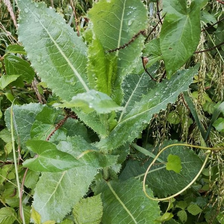
\includegraphics[width=0.3\linewidth]{figuras/foto.png}\hspace{4mm}
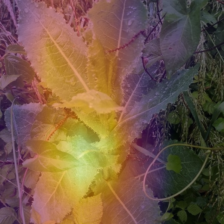
\includegraphics[width=0.3\linewidth]{figuras/mapa.png}\hspace{4mm}
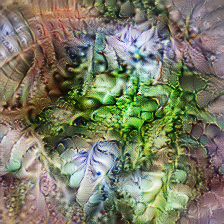
\includegraphics[width=0.3\linewidth]{figuras/patron.png}
\caption{Recorrido completo sobre una misma fotografía. Izquierda: la
entrada, clasificada como \emph{Lactuca serriola} con una probabilidad del
63,0\,\%. Centro: mapa de activación del canal 362 de la última convolución
de la etapa 4, el más activo de esa capa para esta fotografía. Derecha:
imagen optimizada desde ruido para maximizar ese mismo canal.}
\label{fig:pipeline}
\end{figure}

\subsection{Efecto de la robustez a transformaciones}

El artículo sostiene que, sin regularización, la optimización alcanza
activaciones más altas con imágenes peores. Las dos métricas de la
sección~\ref{sec:metricas} permiten comprobarlo de forma cuantitativa. La
tabla~\ref{tab:robustez} compara la optimización de un mismo canal con y
sin robustez a transformaciones.

\begin{table}[!htb]
\centering\small
\caption{Ablación de la robustez a transformaciones. Canal 181 de la última
convolución de la etapa 3, 256 pasos.}
\label{tab:robustez}
\begin{tabular}{l c c}
\toprule
 & \textbf{Activación final} & \textbf{Aspereza} \\
\midrule
Con robustez & $+4{,}93$ & $0{,}164$ \\
Sin robustez & $+7{,}15$ & $0{,}245$ \\
\midrule
Variación & $+45$\,\% & $+49$\,\% \\
\bottomrule
\end{tabular}
\end{table}

Sin robustez, la activación aumenta un 45\,\% y la aspereza un 49\,\%. El
optimizador obtiene un valor mejor del objetivo a costa de una imagen con
más contenido de alta frecuencia, que es el comportamiento descrito en la
sección~\ref{sec:fundamentos}. Desactivar la parametrización de Fourier
también aumenta la aspereza de la imagen final.

%======================================================================
\section{Adaptaciones respecto al artículo}

El artículo aplica sus técnicas a una red GoogLeNet entrenada en ImageNet;
este trabajo las aplica a redes ResNet entrenadas en Pl@ntNet-300K. El número
de pasos se ha reducido de 2560 a 256 por coste, pero puede restablecerse desde
la configuración. Los pesos de las penalizaciones de las figuras del
artículo no son trasladables, porque allí las penalizaciones se suman sobre
todos los elementos de la imagen y aquí se promedian. Por la misma razón,
los pesos de la alineación y de la diversidad se han ajustado con barridos
propios. Por último, el artículo describe una tercera familia de
regularización, los \emph{priors} aprendidos mediante un modelo generativo,
que queda fuera del alcance de este trabajo porque requiere entrenar dicho
modelo.

%======================================================================
\section{Conclusiones}

Se ha aplicado a redes ResNet entrenadas sobre Pl@ntNet-300K el conjunto de
técnicas de visualización de características descrito por Olah et~al.: los
objetivos sobre neuronas, canales, capas y clases; la parametrización en el
dominio de la frecuencia con color decorrelado; la robustez a
transformaciones; las penalizaciones de frecuencia; la interacción entre
neuronas y la diversidad. Sobre ellas se ha construido una herramienta que
relaciona una fotografía con las unidades que activa, con la región donde lo
hace y con el patrón que cada unidad detecta. La ablación de la robustez
confirma de forma cuantitativa que la regularización sacrifica valor del
objetivo a cambio de imágenes interpretables, que es el argumento central
del artículo.

\begin{thebibliography}{9}\small
\bibitem{olah2017} C.~Olah, A.~Mordvintsev y L.~Schubert.
\emph{Feature Visualization}. Distill, 2017. DOI: 10.23915/distill.00007.
\bibitem{plantnet} C.~Garcin, A.~Joly, P.~Bonnet et~al.
\emph{Pl@ntNet-300K: a plant image dataset with high label ambiguity and a
long-tailed distribution}. NeurIPS Datasets and Benchmarks, 2021.
\bibitem{resnet} K.~He, X.~Zhang, S.~Ren y J.~Sun. \emph{Deep Residual
Learning for Image Recognition}. CVPR, 2016.
\bibitem{adam} D.~P.~Kingma y J.~Ba. \emph{Adam: A Method for Stochastic
Optimization}. ICLR, 2015.
\end{thebibliography}

\end{document}
